\documentclass[12pt,a4paper,english]{extarticle}
\usepackage[T1]{fontenc}
\usepackage[utf8]{inputenc}
\usepackage{fourier}
\usepackage{geometry}
\usepackage{multirow}
\geometry{verbose,tmargin=2.2cm,bmargin=2cm,lmargin=2.2cm,rmargin=2cm}
\usepackage{float}
\usepackage{textcomp}
\usepackage{amsmath}
\usepackage{stackrel}
\usepackage{graphicx}
\usepackage{esint}
\usepackage{tikz}
\usetikzlibrary{matrix,calc}

\makeatletter

\providecommand{\tabularnewline}{\\}

\usepackage{fancyhdr}
\usepackage{lscape}
\usepackage{amssymb}
\pagestyle{fancy}
\lhead{Electronica III - 22.13}
\chead{TPL1}
\rhead{ITBA}
\renewcommand{\headrulewidth}{1pt}
\renewcommand{\footrulewidth}{1pt}

\makeatother

\usepackage[english]{babel}

\usepackage{tikz}
\usetikzlibrary{matrix,calc}

%isolated term
%#1 - Optional. Space between node and grouping line. Default=0
%#2 - node
%#3 - filling color
\newcommand{\implicantsol}[3][0]{
    \draw[rounded corners=3pt, fill=#3, opacity=0.3] ($(#2.north west)+(135:#1)$) rectangle ($(#2.south east)+(-45:#1)$);
    }


%internal group
%#1 - Optional. Space between node and grouping line. Default=0
%#2 - top left node
%#3 - bottom right node
%#4 - filling color
\newcommand{\implicant}[4][0]{
    \draw[rounded corners=3pt, fill=#4, opacity=0.3] ($(#2.north west)+(135:#1)$) rectangle ($(#3.south east)+(-45:#1)$);
    }

%group lateral borders
%#1 - Optional. Space between node and grouping line. Default=0
%#2 - top left node
%#3 - bottom right node
%#4 - filling color
\newcommand{\implicantcostats}[4][0]{
    \draw[rounded corners=3pt, fill=#4, opacity=0.3] ($(rf.east |- #2.north)+(90:#1)$)-| ($(#2.east)+(0:#1)$) |- ($(rf.east |- #3.south)+(-90:#1)$);
    \draw[rounded corners=3pt, fill=#4, opacity=0.3] ($(cf.west |- #2.north)+(90:#1)$) -| ($(#3.west)+(180:#1)$) |- ($(cf.west |- #3.south)+(-90:#1)$);
}

%group top-bottom borders
%#1 - Optional. Space between node and grouping line. Default=0
%#2 - top left node
%#3 - bottom right node
%#4 - filling color
\newcommand{\implicantdaltbaix}[4][0]{
    \draw[rounded corners=3pt, fill=#4, opacity=0.3] ($(cf.south -| #2.west)+(180:#1)$) |- ($(#2.south)+(-90:#1)$) -| ($(cf.south -| #3.east)+(0:#1)$);
    \draw[rounded corners=3pt, fill=#4, opacity=0.3] ($(rf.north -| #2.west)+(180:#1)$) |- ($(#3.north)+(90:#1)$) -| ($(rf.north -| #3.east)+(0:#1)$);
}

%group corners
%#1 - Optional. Space between node and grouping line. Default=0
%#2 - filling color
\newcommand{\implicantcantons}[2][0]{
    \draw[rounded corners=3pt, opacity=.3] ($(rf.east |- 0.south)+(-90:#1)$) -| ($(0.east |- cf.south)+(0:#1)$);
    \draw[rounded corners=3pt, opacity=.3] ($(rf.east |- 8.north)+(90:#1)$) -| ($(8.east |- rf.north)+(0:#1)$);
    \draw[rounded corners=3pt, opacity=.3] ($(cf.west |- 2.south)+(-90:#1)$) -| ($(2.west |- cf.south)+(180:#1)$);
    \draw[rounded corners=3pt, opacity=.3] ($(cf.west |- 10.north)+(90:#1)$) -| ($(10.west |- rf.north)+(180:#1)$);
    \fill[rounded corners=3pt, fill=#2, opacity=.3] ($(rf.east |- 0.south)+(-90:#1)$) -|  ($(0.east |- cf.south)+(0:#1)$) [sharp corners] ($(rf.east |- 0.south)+(-90:#1)$) |-  ($(0.east |- cf.south)+(0:#1)$) ;
    \fill[rounded corners=3pt, fill=#2, opacity=.3] ($(rf.east |- 8.north)+(90:#1)$) -| ($(8.east |- rf.north)+(0:#1)$) [sharp corners] ($(rf.east |- 8.north)+(90:#1)$) |- ($(8.east |- rf.north)+(0:#1)$) ;
    \fill[rounded corners=3pt, fill=#2, opacity=.3] ($(cf.west |- 2.south)+(-90:#1)$) -| ($(2.west |- cf.south)+(180:#1)$) [sharp corners]($(cf.west |- 2.south)+(-90:#1)$) |- ($(2.west |- cf.south)+(180:#1)$) ;
    \fill[rounded corners=3pt, fill=#2, opacity=.3] ($(cf.west |- 10.north)+(90:#1)$) -| ($(10.west |- rf.north)+(180:#1)$) [sharp corners] ($(cf.west |- 10.north)+(90:#1)$) |- ($(10.west |- rf.north)+(180:#1)$) ;
}

%Empty Karnaugh map 4x4
\newenvironment{Karnaugh}%
{
\begin{tikzpicture}[baseline=(current bounding box.north),scale=0.8]
\draw (0,0) grid (4,4);
\draw (0,4) -- node [pos=0.7,above right,anchor=south west] {ba} node [pos=0.7,below left,anchor=north east] {dc} ++(135:1);
%
\matrix (mapa) [matrix of nodes,
        column sep={0.8cm,between origins},
        row sep={0.8cm,between origins},
        every node/.style={minimum size=0.3mm},
        anchor=8.center,
        ampersand replacement=\&] at (0.5,0.5)
{
                       \& |(c00)| 00         \& |(c01)| 01         \& |(c11)| 11         \& |(c10)| 10         \& |(cf)| \phantom{00} \\
|(r00)| 00             \& |(0)|  \phantom{0} \& |(1)|  \phantom{0} \& |(3)|  \phantom{0} \& |(2)|  \phantom{0} \&                     \\
|(r01)| 01             \& |(4)|  \phantom{0} \& |(5)|  \phantom{0} \& |(7)|  \phantom{0} \& |(6)|  \phantom{0} \&                     \\
|(r11)| 11             \& |(12)| \phantom{0} \& |(13)| \phantom{0} \& |(15)| \phantom{0} \& |(14)| \phantom{0} \&                     \\
|(r10)| 10             \& |(8)|  \phantom{0} \& |(9)|  \phantom{0} \& |(11)| \phantom{0} \& |(10)| \phantom{0} \&                     \\
|(rf) | \phantom{00}   \&                    \&                    \&                    \&                    \&                     \\
};
}%
{
\end{tikzpicture}
}

%Empty Karnaugh map 2x4
\newenvironment{Karnaughvuit}%
{
\begin{tikzpicture}[baseline=(current bounding box.north),scale=0.8]
\draw (0,0) grid (4,2);
\draw (0,2) -- node [pos=0.7,above right,anchor=south west] {bc} node [pos=0.7,below left,anchor=north east] {a} ++(135:1);
%
\matrix (mapa) [matrix of nodes,
        column sep={0.8cm,between origins},
        row sep={0.8cm,between origins},
        every node/.style={minimum size=0.3mm},
        anchor=4.center,
        ampersand replacement=\&] at (0.5,0.5)
{
                      \& |(c00)| 00         \& |(c01)| 01         \& |(c11)| 11         \& |(c10)| 10         \& |(cf)| \phantom{00} \\
|(r00)| 0             \& |(0)|  \phantom{0} \& |(1)|  \phantom{0} \& |(3)|  \phantom{0} \& |(2)|  \phantom{0} \&                     \\
|(r01)| 1             \& |(4)|  \phantom{0} \& |(5)|  \phantom{0} \& |(7)|  \phantom{0} \& |(6)|  \phantom{0} \&                     \\
|(rf) | \phantom{00}  \&                    \&                    \&                    \&                    \&                     \\
};
}%
{
\end{tikzpicture}
}

%Empty Karnaugh map 2x2
\newenvironment{Karnaughquatre}%
{
\begin{tikzpicture}[baseline=(current bounding box.north),scale=0.8]
\draw (0,0) grid (2,2);
\draw (0,2) -- node [pos=0.7,above right,anchor=south west] {b} node [pos=0.7,below left,anchor=north east] {a} ++(135:1);
%
\matrix (mapa) [matrix of nodes,
        column sep={0.8cm,between origins},
        row sep={0.8cm,between origins},
        every node/.style={minimum size=0.3mm},
        anchor=2.center,
        ampersand replacement=\&] at (0.5,0.5)
{
          \& |(c00)| 0          \& |(c01)| 1  \\
|(r00)| 0 \& |(0)|  \phantom{0} \& |(1)|  \phantom{0} \\
|(r01)| 1 \& |(2)|  \phantom{0} \& |(3)|  \phantom{0} \\
};
}%
{
\end{tikzpicture}
}

%Defines 8 or 16 values (0,1,X)
\newcommand{\contingut}[1]{%
\foreach \x [count=\xi from 0]  in {#1}
     \path (\xi) node {\x};
}

%Places 1 in listed positions
\newcommand{\minterms}[1]{%
    \foreach \x in {#1}
        \path (\x) node {1};
}

%Places 0 in listed positions
\newcommand{\maxterms}[1]{%
    \foreach \x in {#1}
        \path (\x) node {0};
}

%Places X in listed positions
\newcommand{\indeterminats}[1]{%
    \foreach \x in {#1}
        \path (\x) node {X};
}

% \begin{document}
%     \begin{Karnaugh}
%         \contingut{0,0,0,0,0,0,0,0,0,0,0,0,0,0,0,0}
%        \implicant{0}{2}{red}
%        \implicant{5}{15}{purple}
%        \implicantdaltbaix[3pt]{3}{10}{blue}
%     \implicantcantons[2pt]{orange}
%        \implicantcostats{4}{14}{green}
%     \end{Karnaugh}
%     %
%     \begin{Karnaughvuit}
%        \minterms{3,4}
%         \maxterms{0,1,6,7}
%        \indeterminats{2,5}
%        \implicant{3}{2}{green}
%        \implicant{4}{5}{}
%     \end{Karnaughvuit}
%     %
%     \begin{Karnaughquatre}
%         \minterms{1,2}
%        \maxterms{0,3}
%        \implicantsol{1}{green}
%        \implicantsol{2}{red}
%     \end{Karnaughquatre}

% \end{document}

\usepackage{listings}
\newcommand{\horrule}[1]{\rule{\linewidth}{#1}}

\title{
        %\vspace{-1in} 	
        \usefont{OT1}{bch}{b}{n}
        \normalfont \normalsize \textsc{Instituto Tecnológico de Buenos Aires} \\ [25pt]
        \horrule{0.5pt} \\[0.4cm]
        \huge Trabajo Práctico Final \\
        \horrule{2pt} \\[0.5cm]
}
\author{
        \normalfont 								\normalsize
        NOWIK, Ariel 58309\\[-3pt]		\normalsize
        MASPERO, Martina 57120\\[-3pt]		\normalsize
        MESTANZA, Joaquin 58288\\[-3pt]		\normalsize
        REGUEIRA, Marcelo 58300\\[-3pt]		\normalsize
        \today
}
\date{}



%%% Begin document
\begin{document}
% The \input command appends the content of the file directly into the document.
\maketitle
\newpage



\subsection*{Module structure}
\begin{figure}[htbp]
    \begin{center}
    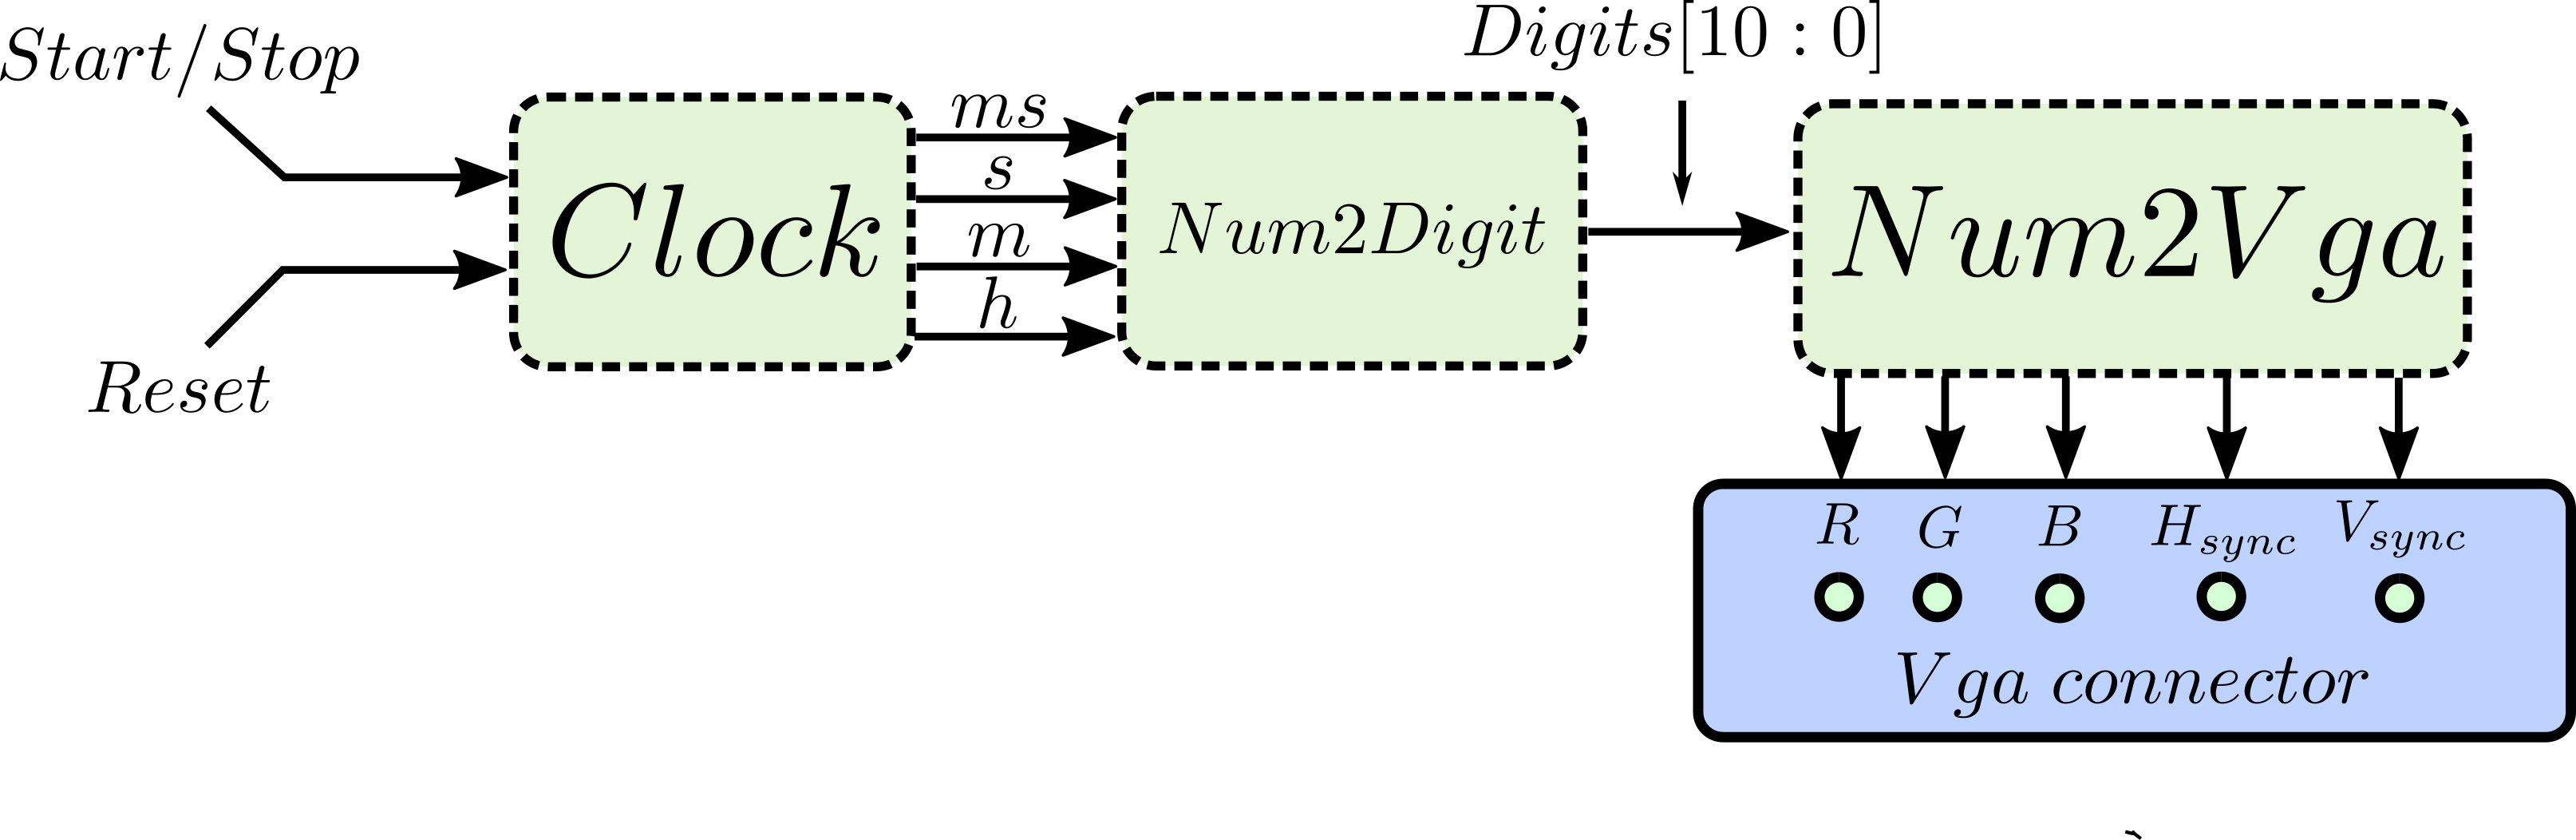
\includegraphics[scale=0.8]{dibujos/estructura.png}
    
    \end{center}
    
    \label{fig:Estructura}
    \end{figure}

The project is organized in three modules:
\begin{enumerate}
\item Clock module: handles the clock reset/start/stop actions (via Buttons), and counts miliseconds, seconds, minutes and hours.
\item Number to digit module: Receives the numbers from the clock and converts them to digit codes.
\item Digit to Screen module: Gets the numbers and handles the Vga protocol. 
\end{enumerate}


\subsection*{Clock syncronization}
\begin{figure}[htbp]
    \begin{center}
    
\includegraphics[scale=0.8]{dibujos/pll.png}
    
    \end{center}
    
    \label{fig:ClockSync}
    \end{figure}

The project uses FPGA internal 50Mhz oscillator. Using two PLLs, the different frequencies needed for each module is generated

\subsection*{Clock Module}

This module recives button input and organizes the counting of the chronometer.
Its output are the numbers of miliseconds, seconds, minutes and hours.
It's implementation is very simple and it is not worth explaining it in detail.

\subsection*{Number to Digit Module}

This module recives the number inputs and converts them to digit codes. That digit code information represent which characetrers will be shown in screen. As there are also ':' character on screen, also there is a digit code 10, that represent that character.
There are, in total 10 digits on screen.

\subsection*{Digit to Screen Module}
This is the most advanced, and difficult to debug module. The objective, however is simple: Show the digits communicated by the digit module on screen one after the other.
When we developed this module we've got a problem. It was not possible, at least directly, to store all 640x800 bits on memory and then access to them, write them, or pass them from one module to another. So we worked hard to find a solution that didn't need that.
The idea is to, in place, when each pixel is drawn, decide, if it will be drawn, or not. We tried to use a simple formula 

\subsubsection*{The magic Lines}
\begin{figure}[htbp]
    \begin{center}
    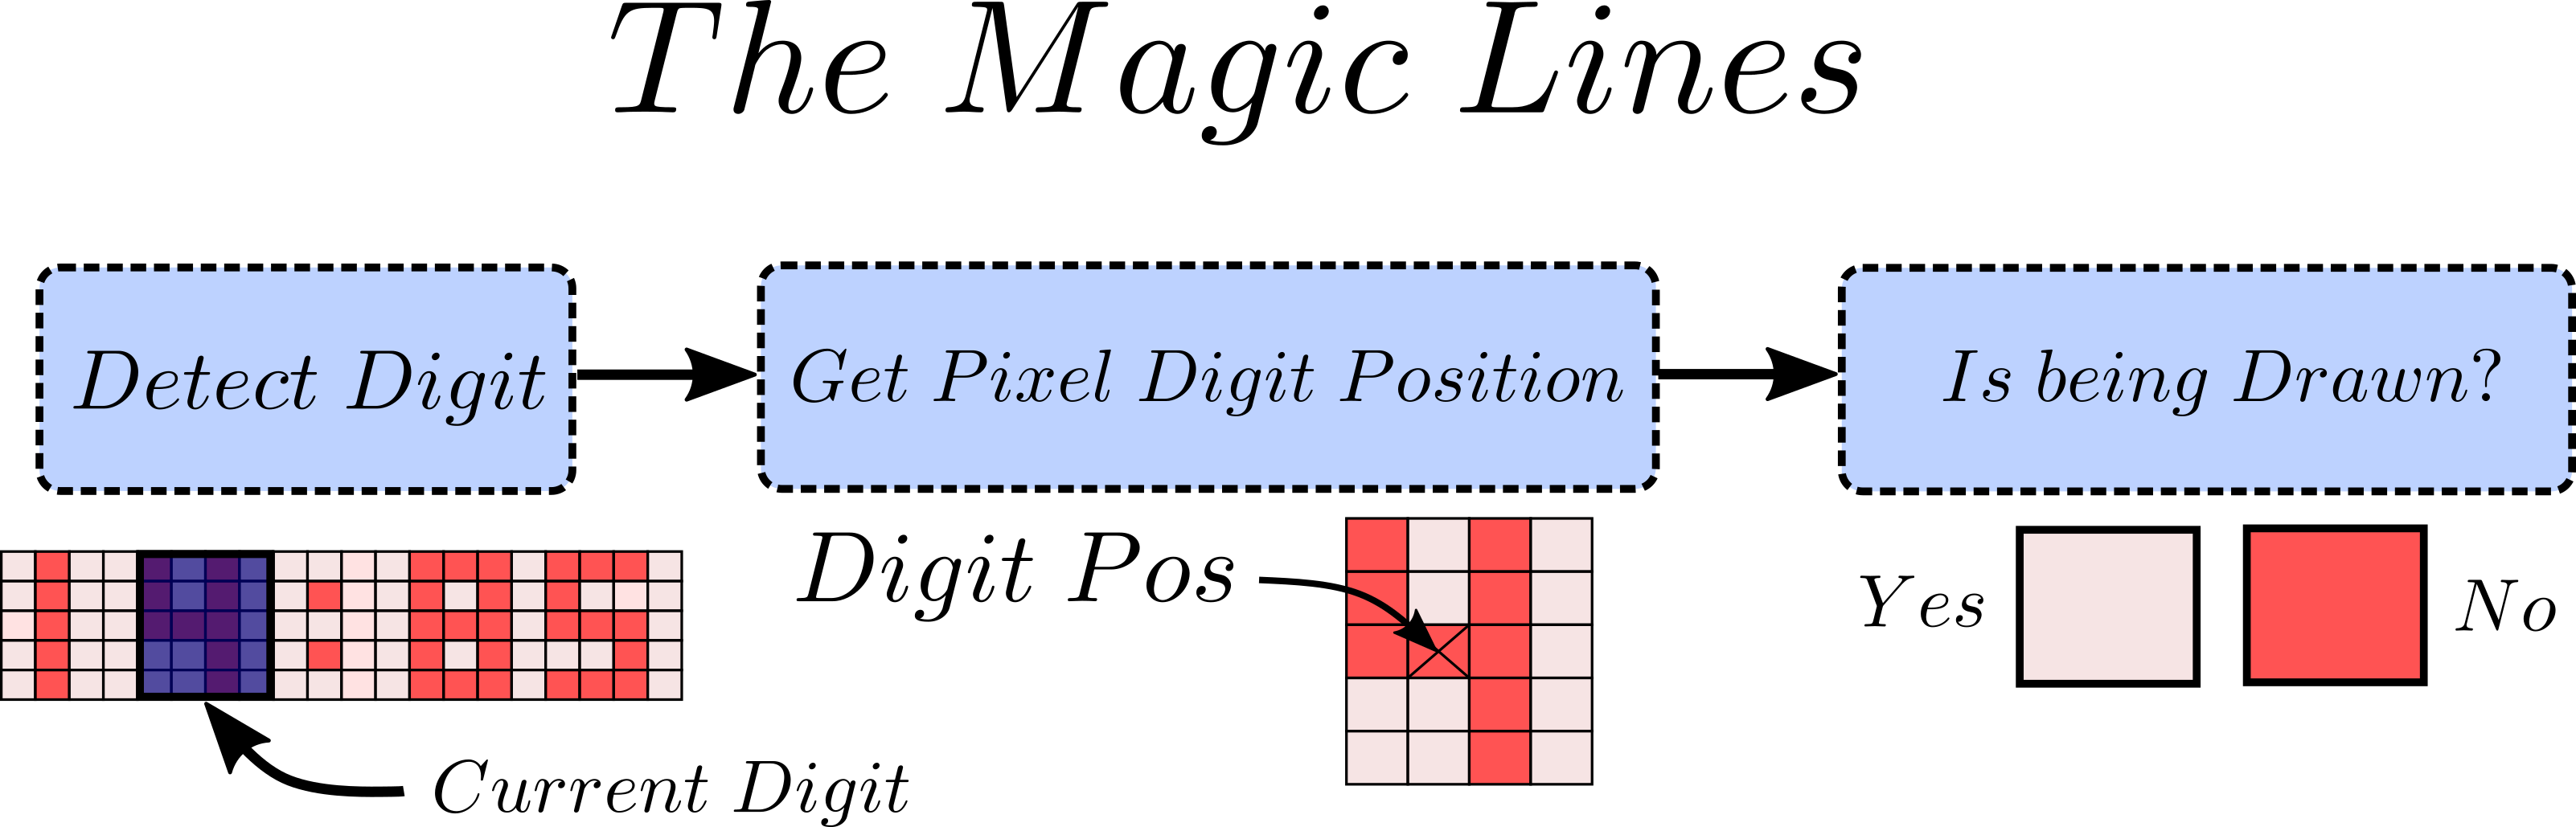
\includegraphics[scale=0.8]{dibujos/digitpng.png}
    
    \end{center}
    
    \label{fig:Magic}
    \end{figure}

We need to do different process when deciding when a digit will be drawn. There are three calculations:
- Detect if we are inside the clock drawing area.

- Detect which digit [0:10] we are drawing. The ':' character count as a one digit

- Detect which position of the digit we are drawing, and the if we are drawing it

These three calculations were done in three lines, thus we gave that lines the name 'the magic lines', they do lot of things in a small part of the code (lines 62, 63 and 64 of display_updater.v)

\subsubsection*{Testing}
We made tests on verilog and gtkwave to check functions of clock and number2digit code, and digit2screen mode. The results were successful.

Here we show a picture of digit2screen module gtkwave output, that was the most interesting

\begin{figure}[htbp]
    \begin{center}
    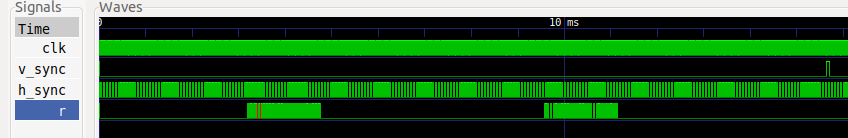
\includegraphics[scale=0.5]{dibujos/digit2screen.png}
    
    \end{center}
    
    \label{fig:Digit2Screen}
    \end{figure}



\subsubsection*{Conclusion}

This was a very challenging project. The hardest part, by far, was making the vga protocol to work, it delayed two days and we've got issues with cable conector. The other parts of the project, were hard, but comparable with the projects done before in the semester 







%%% End document
\end{document}
